%!TEX root = ../CallenThermo.tex
\chapter{其它形式与Legendre变换}
\label{chap5}

\section{能量最小原理}
\label{sec5.1}

在之前的章节中,我们已经得到了熵最大原理的最显著和直接的一些推论。
进一步的推论会导出很多其它有用的基本结论。
不过现在我们重新考虑理论的形式并留意到用一些等价的数学形式可以重新构造出相同的内容,会对促进这些问题的发展更加有用。
这些其它的形式每一个都会在一些特殊类型的问题中显得特别方便,
而热力学计算的艺术大多数情况都体现在选取对于给定的问题最适用的某种理论形式上。
在恰当的形式下热力学问题会变得极为简单,
而在不恰当的形式下问题会变得极为复杂。

力学中也会出现多种等价的形式——Newton形式,Lagrange形式,Hamilton形式是完全等价的。
同样这时也会某一问题用Lagrange形式处理会比用Newton形式更加容易处理的请况,反之亦然。
但是不同形式导致的难易不同在热力学中会表现得极为显著。
正因如此,{\it 等价表述间的变换的普遍性理论被视为热力学理论的一个基础}。

实际上我们已经考虑过了两种等价的表述——能量表述和熵表述。
但基本的极值原理则只在熵表述中被构造出来。
如果这两种表述在理论中的地位是相同的,我们就必须找出能量表述中与熵最大原理类似的极值原理。
这实际上应该是一个与熵最大原理等价的极值原理,并且可以用能量最小原理取代。
熵最大原理告诉我们对于一个给定总能量的平衡态熵会取最大值。
同理,能量最小原理则告诉我们对于给定总熵的平衡态,能量会取最小值。

\begin{figure}[htbp]
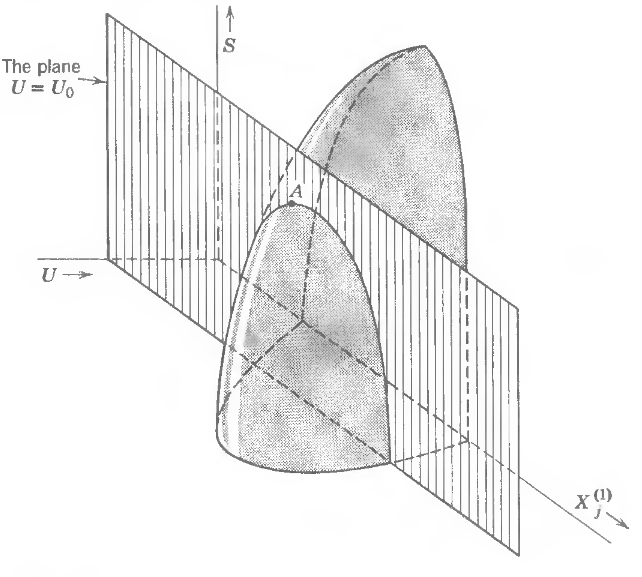
\includegraphics[width=\textwidth]{Pictures/fig5.1.png}
\figcaption{平衡态$A$在给定$U$时$S$取极大。}
\label{fig5.1}
\end{figure}

图\ref{fig5.1}展示了在\ref{sec4.1}节中讨论的复合系统的位形空间的剖面图。
标记为$U$和$S$的轴对应着复合系统的总能量和总熵,而标记为$X_J^{(1)}$的轴则对应着第一个子系统的某个广延参量。
其它没有在图中显示的轴还包括$U^{(1)}$,$X_J$以及其它的$X_K^{(1)}$和$X_K$。

复合系统的总能量是一个由封闭条件决定的常数。
这个封闭条件的几何表示是系统的态处于图\ref{fig5.1}中$U=U_0$的平面上。
系统的基本方程表示为图中的曲面,因此表示系统状态的点一定位于曲面和平面相交得到的曲线上。
如果参数$X_J^{(1)}$不受约束,那么平衡态就是曲线上使得熵最大的态,也就是图\ref{fig5.1}中标记为A的态。

\begin{figure}[htbp]
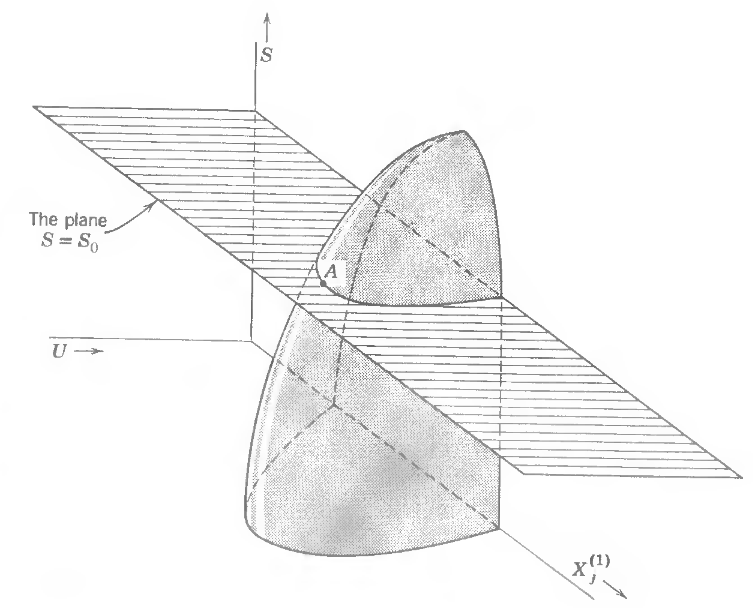
\includegraphics[width=\textwidth]{Pictures/fig5.2.png}
\figcaption{平衡态$A$在给定$S$时$U$取极小。}
\label{fig5.2}
\end{figure}

将平衡态A当做给定熵的时候能量最小态的另一种表述显示在图\ref{fig5.2}中。
经过平衡态点A的平面$S=S_0$与基本曲面相交定义了一条曲线。
这条曲线包含了一族熵为常数的态,{\it 而平衡态A则是曲线上使得能量最小的态}。

如同图\ref{fig5.1}和\ref{fig5.2}所示,熵最大和能量最小原理的等价性明确依赖于基本曲面\mpar{基本方程所对应的曲面}的几何形状这个性质,是普遍的。
如同\ref{sec4.1}节中讨论过的那样,图中显示的曲面的形状是由$\partial S/\partial U>0$以及$U$是关于$S$的单值连续函数这两个假设决定的;
因此这两个解析的假设是两个原理等价的隐含条件。

总结一下,尽管我们尚未证明,但看起来以下两个原理是等价的:

{\bf 熵最大原理.}{\it 在总的内部能量确定时,任何不受约束的参数在平衡时的取值都使得熵最大}。

{\bf 能量最小原理.}{\it 在总的熵确定时,任何不受约束的参数在平衡时的取值都使得能量最小}。

两个极值准则的等价性的证明即可以用物理论证的方式阐述,也可以用数学证明的方式阐述。
我们首先考虑物理讨论,来论证如果能量{\it 不}是最小值的话那么熵就可以不是最大值,并且反之亦然。

接下来,假设系统处于平衡态但能量并{\it 不}是在给定的熵下可能的最小的值。
我们就可以在保持熵为常数的同时从系统中提取能量(用功的形式),并且我们随后就可以用热量的形式把这部分能量返回
这样系统的熵会增加($\dbar Q=T\,\mathrm dS$),并且系统会恢复到它初始的能量但是熵增加了。
这跟初始的平衡态是熵最大的态是矛盾的!
因此我们不得不推断最初的平衡态必须具有给定的熵下最小的能量。

相反的推论,也就是最小能量要求最大的熵,可以用类似的方式构造(见问题 \ref{pro5.1-1}).

在更形式化的证明中,我们假设熵最大原理表述为
\begin{equation}
\label{equ5.1}
\left(\frac{\partial S}{\partial X}\right)_U=0
~\text{及}~
\left(\frac{\partial^2 S}{\partial X^2}\right)_U<0
\end{equation}
在此为了简便,我们将$X_J^{(1)}$写作$X_J$,这暗示着其它的$X$将保持为常数。
同时为了简便,我们暂时将一阶导数$(\partial U/\partial U)_S$记为$P$。
于是根据(根据附录\ref{appendix.A}中的公式\eqref{equA.22})

\begin{equation}
\label{equ5.2}
	P \equiv \left( \frac{\partial U}{\partial X} \right)_S = -\frac{\left( \frac{\partial S}{\partial X} \right)_U }{ \left( \frac{\partial S}{\partial U}\right)_X } = -T \left(\frac{\partial S}{\partial X}\right)_U = 0
\end{equation}

我们得到$U$是极值。
为了分清这个极值是极大极小还是一个拐点,我们必须研究二阶导数$(\partial^2U/\partial X^2)_S\equiv(\partial P/\partial X)_S$的符号。
但是如果将$P$当做$U$和$X$的函数,我们有
\begin{align}
\label{equ5.3}
\left(\frac{\partial^2 U}{\partial X^2}\right)_S
&=\left(\frac{\partial P}{\partial X}\right)_S
=\left(\frac{\partial P}{\partial U}\right)_X
\left(\frac{\partial U}{\partial X}\right)_S
+\left(\frac{\partial P}{\partial X}\right)_U
=\left(\frac{\partial P}{\partial U}\right)_XP
+\left(\frac{\partial P}{\partial X}\right)_U \\
\label{equ5.4}
&=\left(\frac{\partial P}{\partial X}\right)_U.~\text{若}P=0
\end{align}

\begin{equation}
\label{equ5.5}
=\frac{\partial}{\partial X}
\left[-\frac{\left(\frac{\partial S}{\partial X}\right)_U}{\left(\frac{\partial S}{\partial U}\right)_X}\right]_U
\end{equation}

\begin{equation}
\label{equ5.6}
=-\frac{\frac{\partial^2S}{\partial X^2}}
{\frac{\partial S}{\partial U}}+\frac{\partial S}{\partial X}
\frac{\frac{\partial^2S}{\partial X\partial U}}{\left(\frac{\partial S}{\partial U}\right)^2}
\end{equation}

\begin{equation}
\label{equ5.7}
=-T\frac{\partial^2S}{\partial X^2}>0
~\text{若}\frac{\partial S}{\partial X}=0
\end{equation}
因此$U$是一个极小值。
反向的论证在形式上是一样的。

如同以上所指出的,两个极值条件描述的情形是完全一样的这一事实类似于几何中的等周问题。
也就是一个圆既可以描述为给定周长下面积最大的二维图形,也可以描述为给定面积下周长最小的二维图形。


两个可供选择的用于描述圆的极值条件是完全等价的,而且每一个都适用于所有的圆。
不过他们给出两种不同的生成圆的方法。
假设我们有一个正方形并且想使它连续变形为一个圆。
我们可以保持它的面积是常数并且允许约束的曲线像橡皮筋一样收缩。
这样我们得到了作为给定面积下周长最小图形的一个圆。
等价地,我们也可以保持正方形的周长不变并允许面积增加,这样我们就得到了作为给定周长下面积最大图形的一个(不同的)圆。
尽管如此,在得到这些圆之后,{\it 每一个圆都同时满足自身取值下面积和周长的极值条件}。

关于热力学系统的物理情形跟上面描述的几何的情形是非常类似的。
也就是说,任何一个平衡态既可以描述为给定能量下熵最大的态,也可以描述为给定熵下能量最小的态。
但是这两个条件却给出了两个不同的达到平衡态的方法。
作为这两种接近平衡的方法的一个特定的例子,考虑一个初始位于一个封闭圆柱的某个位置的活塞。
我们的兴趣在于不通过约束活塞位置来使系统达到平衡。
我们可以简单地移去约束来使它自发达到平衡;此时由于封闭条件,能量会保持为常数而熵会增加。
这个过程就是熵最大原理所要求的过程。
等价地,我们可以让活塞非常缓慢地移动,可逆地对外做功直到它到达使两边压强相等的位置。
在这个过程中能量被从系统中提取出来,但是它的熵保持为常数(这个过程是可逆的且没有热流)。
这个过程就是能量最小原理要求的过程。
我们想强调的关键事实是,{\it 与通过二者之一或是其它的某种过程达到平衡态的具体过程无关,通过各种方式达到的最终的平衡态都满足两种极值条件}%
\mpar{当然,从一个初态出发,通过不同的过程会到达不同的平衡态。}%
。

最后我们通过以能量最小原理替代熵最大原理来解决\ref{sec2.4}节中的热平衡问题来阐明它。
我们考虑一个内部具有一个导热的刚性隔离墙的封闭的复合系统。
热量可以在两个子系统间自由流动,因此我们想找到它的平衡态。
在能量表述下的基本方程是
\begin{equation}
\label{equ5.8}
U=U^{(1)}(S^{(1)},V^{(1)},N^{(1)}_1,\ldots)+U^{(2)}(S^{(2)},V^{(2)},N^{(2)}_1,\ldots)
\end{equation}
所有的关于体积和摩尔数的参数都是已知的常数。
需要被计算的变量是$S^{(1)}$和$S^{(2)}$。
现在,忽略系统封闭导致的总能量不变的事实,{\it 如果}能量的改变被允许的话,平衡态可以被表示为使得能量最小的态。
总能量关于两个系统中虚拟热流的虚拟变化是
\begin{equation}
\label{equ5.9}
\,\mathrm dU=T^{(1)}\,\mathrm dS^{(1)}+T^{(2)}\,\mathrm dS^{(2)}
\end{equation}
能量最小条件也就是$dU=0$,在服从总熵不变的条件时:
\begin{equation}
\label{equ5.10}
S^{(1)}+S^{(2)}=\text{constant}
\end{equation}
会有
\begin{equation}
\label{equ5.11}
\mathrm dU=(T^{(1)}-T^{(2)})\,\mathrm dS^{(1)}=0
\end{equation}
于是我们可以推出
\begin{equation}
\label{equ5.12}
T^{(1)}=T^{(2)}
\end{equation}

从而能量最小原理对我们给出了与我们前面用熵最大原理得到的相同的热平衡条件。

方程\eqref{equ5.12}是一个关于$S^{(1)}$和$S^{(2)}$的方程。
在总能量$U$已知,因此仅有的两个未知量是$S^{(1)}$和$S^{(2)}$的情况下,第二个方程选为方程\eqref{equ5.8}最为方便。
理论上方程\eqref{equ5.8}和\eqref{equ5.12}会给出这个问题的精确解。

用完全一样的思路,可以发现一个内部带有可动绝热墙的封闭系统的平衡条件是压强相等。
这个结论在能量表述中是非常直接的,但是如同在\ref{sec2.7}的最后一段看到的,在熵表述中相对更加微妙。

\section{Legendre变换}
\label{sec5.2}

在能量表述和熵表述中,广延量都表现为数学上的独立变量,而强度量都看成被导出的物理量。
这个情形跟实验室中更方便的实际情况中的需求形成了对比。
实验者经常发现强度量更容易测量和控制,因此更喜欢把强度量当成操作上的独立变量而把广延量当成导出量。
极端情况是熵和温度这一对共轭变量:
并不存在可以测量和控制熵的实验仪器,而用来测量和控制温度的温度计和恒温器在实验室中则是非常常见的。
随之而来的问题就是,能否改变数学形式使得强度量代替广延量成为数学上的独立变量。
我们会看到这种重新表述是可行的,而且还可以导出很多其它形式的热力学表述。

重说三:不论是在熵表述还是能量表述下热力学都是逻辑完备且独立的,而介绍这些变换表述纯粹只是为了方便。
这被公认为是一种使热力学避免了无用的尴尬的简化方法。但是原则上讲这只是某种捷径,并不是逻辑上所必须的。

接下来我们给出这个问题纯粹的形式化表述。
我们有一个形如
\begin{equation}
\label{equ5.13}
  Y=Y(X_0,X_1,\ldots,X_l)
\end{equation}
的方程(基本关系),并且想找到一个将导数
\begin{equation}
\label{equ5.14}
  P_k\equiv\frac{\partial Y}{\partial X_k}
\end{equation}
作为独立变量,但是不改变给出的基本关系\eqref{equ5.13}中任何其他信息的方法。
形式上,在几何和其他一些物理领域中也有与之类似的问题。
这个问题的解答需要采用名为Legendre变换的数学技术,如果给出它的几何表述的话会最为直观。
在这一节中我们就会给出这个几何表述。

\begin{figure}[htbp]
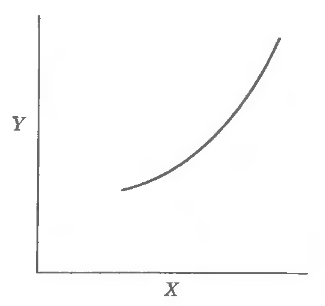
\includegraphics[width=.5\textwidth]{Pictures/fig5.3.png}
\figcaption{}
\label{fig5.3}
\end{figure}

简便起见,我们首先考虑基本关系使只关于一个独立变量$X$的函数的数学情形。
\begin{equation}
\label{equ5.15}
  Y=Y(X)
\end{equation}
几何上,这个基本关系可以被表现为具有笛卡尔坐标$X$和$Y$的空间中的一条曲线(图\ref{fig5.3}),而导数
\begin{equation}
\label{equ5.16}
  P\equiv\frac{\partial Y}{\partial X}
\end{equation}
是这个曲线的斜率。
现在如果我们想用$P$代替$X$作为一个独立变量,我们的第一反应可能是简单地用方程\eqref{equ5.15}和\eqref{equ5.16}消去$X$,
从而得到$Y$关于$P$的函数
\begin{equation}
\label{equ5.17}
  Y=Y(P)
\end{equation}
从几何上来看,我们立刻会发现,这样做无论如何都会在数学上牺牲掉给出的基本关系\eqref{equ5.15}的一些信息。
显然对于$Y$关于斜率$dY/dX$的函数的了解并不能让我们重构出曲线$Y=Y(X)$。
实际上图\ref{fig5.4}中每一条替代的曲线都等价地满足关系$Y=Y(P)$。
从分析的观点来看,关系$Y=Y(P)$是一个一阶微分方程,而它的积分给出的结果跟$Y=Y(X)$只差一个待定的积分常数。
因此我们看到,如果用$Y=Y(P)$代替$Y=Y(X)$成为基本方程,就会导致丢失掉基本关系中的一些原始信息。
尽管我们希望让$P$成为一个数学上的独立变量,但形式中包含的信息的丢失却是完全不可接受的。

\begin{figure}[htbp]
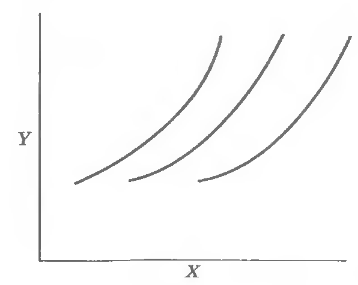
\includegraphics[width=\textwidth]{Pictures/fig5.4.png}
\figcaption{}
\label{fig5.4}
\end{figure}

问题的实际的解是由传统的{\it 点几何(point geometry)}与Pluecker的{\it 线几何(line geometry)}的对偶关系给出的。
线几何中的基本概念是一条给定的曲线可以很好地由以下两种方式等价描述:
(a) 作为一族切线的包络线(图\ref{fig5.5});
(b) 作为满足关系$Y=Y(X)$的点的轨迹。
任何可以使我们构造出一族切线的方程都能和关系$Y=Y(X)$一样好地决定一条曲线。

\begin{figure}
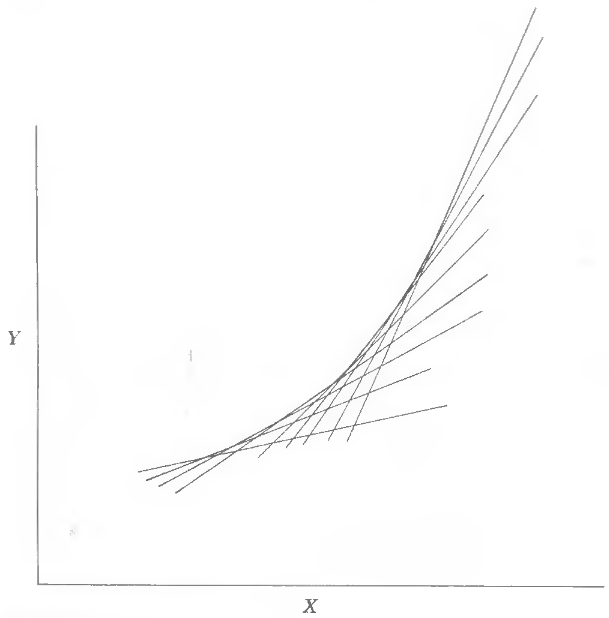
\includegraphics[width=\textwidth]{Pictures/fig5.5.png}
\figcaption{}
\label{fig5.5}
\end{figure}

正如平面上的每一个点都可以由两个数$X$和$Y$描述,平面上的每一条直线也都可以用两个数$P$和$\psi$描述,
其中$P$是直线的斜率,$\psi$是它在$Y$轴上的截距。
于是正如关系$Y=Y(X)$挑出了所有可能的点$(X,Y)$中的一个子集,
关系$\psi=\psi(P)$挑出了所有可能的直线$(P,\psi)$的一个子集。
关于切线的截距$\psi$作为斜率$P$的函数的知识可以让我们构造出一族切线,
从而也就构造出了它们的包络线也就是这条曲线。
因此关系
\begin{equation}
\label{equ5.18}
  \psi=\psi(P)
\end{equation}
是跟基本关系$Y=Y(X)$完全等价的。
在这个关系中,独立变量是$P$,于是方程\eqref{equ5.18}给出了对于这个问题的一个满足要求的完备的解。
由于关系$\psi=\psi(P)$跟关系$Y=Y(X)$是数学等价的,所以它也可以被当成一个基本关系;
$Y=Y(X)$是“$Y$表述”下的基本关系,而$\psi=\psi(P)$是“$\psi$表述”下的基本关系。

在这里我们建议读者去画一些具有不同的斜率$P$和不同的$Y$轴截距$\psi=-P^2$的直线。
可以看出关系$\psi=-P^2$描述了一条抛物线(更加一般的描述是$Y=\frac{1}{4}X^2$)。
在“$\psi$表述”下抛物线的基本方程是$\psi=-P^2$,而“$Y$表述”下同一条抛物线的基本方程是$Y=\frac{1}{4}X^2$。

\begin{figure}[htbp]
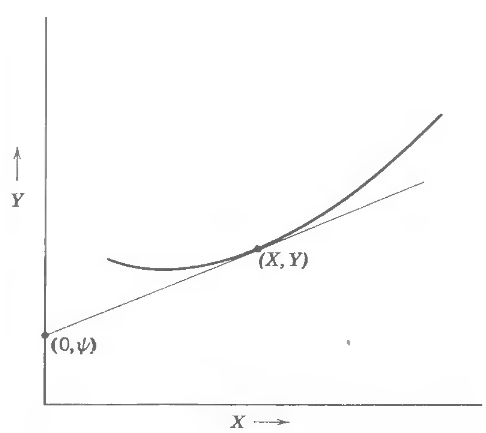
\includegraphics[width=.7\textwidth]{Pictures/fig5.6.png}
\figcaption{}
\label{fig5.6}
\end{figure}

现在面临的问题就是如果我们给出关系$Y=Y(X)$后如何计算出关系$\psi=\psi(P)$。
恰当的数学操作被称为Legendre(Legendre)变换。
我们考虑一条经过点$(X,Y)$斜率为$P$的切线。
如果截距是$\psi$,我们有(见图\ref{fig5.6})
\begin{equation}
\label{equ5.19}
  P=\frac{Y-\psi}{X-0}
\end{equation}
或者
\begin{equation}
\label{equ5.20}
  \psi=Y-PX
\end{equation}

现在我们假设我们已经有方程
\begin{equation}
\label{equ5.21}
  Y=Y(X)
\end{equation}
并且通过求导我们可以得到
\begin{equation}
\label{equ5.22}
  P=P(X)
\end{equation}
于是通过在方程\eqref{equ5.20},\eqref{equ5.21}和\eqref{equ5.22}消除掉%
\footnote{在$P$不是与$X$无关的情况下这个消除是可以做到的,也就是要求$d^2Y/dX^2\neq0$。
应用到热力学上,这等价于稳定性的要求。
这个标准只有在“临界点”才会失效,这会在第\ref{chap10}章里讨论。}%
$X$和$Y$我们就能得到想要的$\psi$和$P$之间的关系。
Legendre(Legendre)变换的基本等式就是方程\eqref{equ5.20},
而这个方程可以被当成函数$\psi$的解析定义。
函数$\psi$被称为$Y$的{\it Legendre变换(Legendre transformation)}。

相反的问题是如果给出关系$\psi=\psi(P)$的话重新求出关系$Y=Y(X)$。
我们可以看出在这里$(X,Y)$和$(\psi,P)$之间的关系跟它的逆关系是对称的,
区别只是Legendre的方程中差了一个符号。
对方程\eqref{equ5.20}求导并且应用$\,\mathrm dY=P\,\mathrm dX$,我们可以发现
\begin{eqnarray}
\label{equ5.23}
  \,\mathrm d\psi &=& \,\mathrm dY-P\,\mathrm dX-X\,\mathrm dP \nonumber \\
  ~ &=& -X\,\mathrm dP
\end{eqnarray}
或者
\begin{equation}
\label{equ5.24}
  -X=\frac{\mathrm d\psi}{\mathrm dP}
\end{equation}
如果从给出的方程$\psi=\psi(P)$和方程\eqref{equ5.24}和\eqref{equ5.20}中消除掉%
\footnote{这样做可能的条件是$d^2\psi/dP^2\neq0$,在热力学中是由所考虑的系统的稳定性保证的。}%
两个变量$\psi$和$P$,我们就重构出了关系$Y=Y(X)$。
Legendre变换和它的逆的对称性可以通过下面的对比表显示出来:
\begin{equation*}
\begin{array}{c|c}
\hline
Y=Y(X) & \psi=\psi(P) \\
P=\frac{\mathrm dY}{\mathrm dX} & -X=\frac{\mathrm d\psi}{\mathrm dP} \\
\psi=-PX+Y & Y=XP+\psi \\
\text{消掉$X$和$Y$得到} & \text{消掉$P$和$\psi$得到} \\
\psi=\psi(P) & Y=Y(X)\\
\hline
\end{array}
\end{equation*}

将Legendre变换推广到关于不止一个以及独立变量的函数是简单直接的。
在三维中,$Y$是关于$X_0$和$X_1$的函数,同时基本方程表述了一个曲面。
这个曲面可以被当成满足基本方程$Y=Y(X_0,X_1)$的点的轨迹,或者被当成切平面的包络面。
一个平面可以用在在$Y$轴上的截距$\psi$和在$Y-X_0$以及$Y-X_1$平面上的截线的斜率$P_0$和$P_1$来刻画。
于是基本方程就是所有可能的平面中用$\psi=\psi(P_0,P_1)$描述的子集。

一般地给出的基本关系
\begin{equation}
\label{equ5.25}
  Y=Y(X_0,X_1,\dots,X_t)
\end{equation}
表示了一个在具有笛卡尔坐标$Y,X_0,X_1,\dots,X_t$的$(t+2)$维空间中的超平面。
导数
\begin{equation}
\label{equ5.26}
  P_k=\frac{\partial Y}{\partial X_k}
\end{equation}
是曲面的偏斜率。
超曲面可以等价地用满足方程\eqref{equ5.25}描述的点的轨迹或者切超平面的包络来描述。
切超平面族可以用超平面的截距$\psi$关于斜率$P_0,P_1,\dots,P_t$的函数来刻画。
于是
\begin{equation}
\label{equ5.27}
  \psi=Y-\sum_kP_kX_k
\end{equation}
对这个方程求微分,我们可以发现
\begin{equation}
\label{equ5.28}
  \,\mathrm d\psi=-\sum_kX_k\,\mathrm dP_k
\end{equation}
从而
\begin{equation}
\label{equ5.29}
	-X_k = \frac{\partial \psi}{\partial P_k}
\end{equation}
Legendre变换实现了从$Y=Y(X_0,X_1,\dots,X_t)$,方程组\eqref{equ5.26}和方程\eqref{equ5.27}中消去$Y$和$X_k$。
逆变换实现了从从$\psi=\psi(P_0,P_1,\dots,P_t)$,方程组\eqref{equ5.29}和方程\eqref{equ5.27}中消去$Y$和$X_k$。

最后,Legendre变换可以仅仅在关系$Y=Y(X_0,X_1,\dots,X_t)$的$(t+2)$维全空间中的一个$(n+2)$维子空间中进行。
显然这个子空间必须包含$Y$坐标,但是可以包含集合$X_0,X_1,\dots,X_t$中的任选$n+1$个坐标。
为了记号上的方便,我们排列坐标使得Legendre变换作用在前$n+1$个坐标(以及$Y$)构成的子空间上;
坐标$X_{n+1},X_{n+2},\dots,X_t$保持不变。
这样一个部分Legendre变换的作用只不过是在变幻中把$X_{n+1},X_{n+2},\dots,X_t$当成常数。
得到的Legendre变换必须用一些精确的符号标记标出哪些独立变量参与了变换。
我们引入标记$Y[P_0,P_1,\dots,P_n]$来标记对函数$Y(X_0,X_1,\dots,X_t)$做对应于$X_0,X_1,\dots,x_n$的Legendre变换。
从而$Y[P_0,P_1,\dots,P_n]$就是一个关于独立变量$P_0,P_1,\dots,P_n,X_{n+1},\dots,X_t$的函数。
在接下来的表中展示了在部分Legendre变换和它的逆变换中包含的各种关系。
\begin{tabularx}{\textwidth}{X|X}
\hline
  $Y=Y(X_0,X_1,\dots,X_t)$ & \begin{mymath}Y[P_0, P_1, \dots, P_n] = P_0, P_1, \dots, P_n, X_{n+1}, \dots, X_t \, \text{的函数}\label{equ5.30}\end{mymath}\\
  $P_k = \frac{\partial Y}{\partial X_k}$ & \begin{mymath}-X_k = \frac{\partial Y[P_0,\dots,P_n]}{\partial P_k}, \quad k\leq n\label{equ5.31}\end{mymath} \\
   & $P_k = \frac{\partial Y[P_0,\dots,P_n]}{\partial X_k}\quad k > n$ \\
  偏微分表示了$Y$的所有除了$X_k$以外的自然变量(比如所有满足$j\neq k$的$X_j$) & 偏微分表示了$Y[P_0,\dots,P_n]$除了已经包含了其偏微分以外的所有自然变量。 \\
  $\,\mathrm dY=\sum_0^t P_k\,\mathrm dX_k$ & \begin{mymath}\mathrm dY[P_0, \dots, P_n] = -\sum_0^n X_k \,\mathrm dP_k + \sum_{n + 1}^t P_k \,\mathrm dX_k \label{equ5.32}\end{mymath}\\
  $Y[P_0,\dots,P_n]=Y-\sum_0^nP_kX_k$ & \begin{mymath}Y=Y[P_0,\dots,P_n]+\sum_0^nX_kP_k\label{equ5.33}\end{mymath} \\
  从方程(5.30),(5.33)和(5.31)的前$n+1$个方程中消除掉$Y$和$X_0, X_1,\dots,X_n$可以导出变换后的基本关系。 & 从方程(5.30),(5.33)和(5.31)的前$n+1$个方程中消除掉$Y[P_0, \dots, P_n]$和$P_0, P_1, \dots, P_n$可以导出原始的基本关系。\\
  \hline
\end{tabularx}

在这一节中我们已经将Legendre变换的数学形式和物理应用分离开来。
在开始下一节继续热力学的应用之前,指出其在物理学中相比热力学更让人熟知的一个领域——Lagrangian和Hamiltonian力学中的应用,将是富有教益的。
而这或许是物理学中除了热力学以外最熟悉的领域。
Lagrange原理宣称,存在一个特殊的函数Lagrange量,完整地刻画了一个力学系统的动力学。
Lagrange量是一个关于$2r$个变量的函数,其中$r$个是{\it 广义坐标(generalized coordinates)},$r$个是{\it 广义速度(generalized velocities)}。因此方程
\begin{equation}
\label{equ5.34}
  L=L(v_1,v_2,\dots,v_r,q_1,q_2,\dots,q_r)
\end{equation}
扮演了基本关系的角色。{\it 广义动量(generalized momenta)}被定义成拉氏量的导数
\begin{equation}
\label{equ5.35}
	P_k \equiv \frac{\partial L}{\partial v_k}
\end{equation}
如果想要用动量代替速度作为独立变量,我们必须做关于速度的部分Legendre变换。
从而我们引入一个新的函数,叫做Hamilton量,定义是%
\footnote{我们约定Lagrange量的Legendre变换是{\it 负}的Hamilton量。实际上,数学上的约定和力学中的是一样的,而函数$-\psi$会被叫做$Y$的Legendre变换}%
\begin{equation}
\label{equ5.36}
  (-H)=L-\sum_1^rP_kv_k
\end{equation}
然后一个完整的动力学形式就可以基于这个新的基本关系给出
\begin{equation}
\label{equ5.37}
  H=H(P_1,P_2,\dots,P_r,q1,q2,\dots,q_r)
\end{equation}
此外,根据方程\eqref{equ5.31}$H$的关于$P_k$的导数是速度$v_k$,也就是Hamilton动力学方程之一。
因此如果形如\eqref{equ5.34}的一个方程被当成Lagrangian表述的动力学方程,那么Hamilton方程\eqref{equ5.37}就是Hamiltonian表述中等价的基本方程。



\section{热力学势}
\label{sec5.3}

前面介绍的形式在热力学中的应用是不言自明的。
基本关系$Y=Y(X_0,X_1,\dots)$可以被解释为能量表述的基本关系$U=U(S,X_1,X_2,\dots,X_t)$或者$U=U(S,V,N_1,N_2,\dots)$。
而偏导数$P_0,P_1,\dots$对应着强度量$T,-P,\mu_1,\mu_2,\dots$。
Legendre(Legendre)变换后的函数被叫做{\it 热力学势},而现在我们明确定义它们中最常见的几个。
在第\ref{chap6}章中将通过得到每一个势的极值原理继续关于这些函数的讨论,表明每一个的直观意义,并且讨论在热力学理论中它们的特殊角色。
但现在我们关注几个特定的函数的形式化定义。

{\it Helmholtz势(Helmholtz potential)}或者{\it Helmholtz自由能(Helmholtz free energy)},是$U$用温度代替熵成为独立变量的Legendre变换。
按国际标准,Helmholtz势的符号是$F$。
Helmholtz势的自然变量是$T,V,N_1,N_2,\dots$。
也就是函数关系$F=F(T,V,N_1,N_2,\dots)$构成一个基本关系。
在\ref{sec5.2}节中的系统记号
\begin{equation}
\label{equ5.38}
  F\equiv U[T]
\end{equation}

能量表述和亥姆霍兹(Helmholtz)表述的完整关系,总结在了下面的对比表中:

\begin{tabular}{c|c}
\hline
$U=U(S,V,N_1,N_2,\dots)$ & \begin{mymath}F=F(T,V,N_1,N_2,\dots)\label{equ5.39}\end{mymath}\\
$T=\partial U/\partial S$ & \begin{mymath}-S=\partial F/\partial T\label{equ5.40} \end{mymath}\\
$F=U-TS$ & \begin{mymath}U=F+TS \label{equ5.41} \end{mymath}\\
消去$U$和$S$得到 & 消去$F$和$T$得到\\
$F=F(T,V,N_1,N_2,\dots)$ & $U=U(S,V,N_1,N_2,\dots)$\\
\hline
\end{tabular}

全微分$\mathrm dF$是
\begin{equation}
\label{equ5.42}
  \,\mathrm dF=-S\,\mathrm dT-P\,\mathrm dV+\mu_1\,\mathrm dN_1+\mu_2\,\mathrm dN_2+\cdots
\end{equation}

{\it 焓(enthalpy)}是$U$用压强代替体积成为独立变量的部分Legendre变换。
按照国际物理学会和化学学会的建议,以及跟基本上普适的用法保持一致,我们用符号$H$来标记焓。
这个势的自然变量是$S,P,N_1,N_2,\dots$而且
\begin{equation}
\label{equ5.43}
  H\equiv U[P]
\end{equation}
表示能量和焓表述的关系的表如下

\begin{tabular}{c|c}
\hline
$U=U(S,V,N_1,N_2,\dots)$ & \begin{mymath}H=H(S,P,N_1,N_2,\dots)\label{equ5.44}\end{mymath}\\
$-P=\partial U/\partial V$ & \begin{mymath}V=\partial H/\partial P\label{equ5.45} \end{mymath}\\
$H=U+PV$ & \begin{mymath}U=H-PV \label{equ5.46} \end{mymath}\\
\text{消去$U$和$V$得到} & \text{消去$H$和$P$得到}\\
$H=H(S,P,N_1,N_2,\dots)$ & $U=U(S,V,N_1,N_2,\dots)$\\
\hline
\end{tabular}

需要特别注意的是方程\eqref{equ5.45}和\eqref{equ5.46}的符号的反转,
导致了$-P$成为了对应$V$的强度量。
全微分$\,\mathrm dH$是
\begin{equation}
\label{equ5.47}
  \,\mathrm dH=T\,\mathrm dS+V\,\mathrm dP+\mu_1\,\mathrm dN_1+\mu_2\,\mathrm dN_2+\dots
\end{equation}

第三个常用的能量的Legendre变换是{\it Gibbs势(Gibbs potential)}或者叫{\it Gibbs自由能(Gibbs free energy)}。
这个势是同时用温度代替熵并用压强代替体积作为独立变量的Legendre变换.
标准的记号是$G$,而自然变量是$T,P,N_1,N_2,\dots$。
从而我们有
\begin{equation}
\label{equ5.48}
  G\equiv U[T,P]
\end{equation}
以及

\begin{tabular}{c|c}
\hline
$U=U(S,V,N_1,N_2,\dots)$ & \begin{mymath}G=G(T,P,N_1,N_2,\dots)\label{equ5.49}\end{mymath}\\
$T=\partial U/\partial S$ & \begin{mymath}-S=\partial G/\partial T\label{equ5.50} \end{mymath}\\
$-P=\partial U/\partial V$ & \begin{mymath}V=\partial G/\partial P\label{equ5.51} \end{mymath}\\
$G=U-TS+PV$ & \begin{mymath}U=G+TS-PV \label{equ5.52} \end{mymath}\\
消去$U$,$S$和$V$得到 & 消去$H$,$T$和$P$得到\\
$G=G(T,P,N_1,N_2,\dots)$ & $U=U(S,V,N_1,N_2,\dots)$\\
\hline
\end{tabular}

全微分$\,\mathrm dG$是
\begin{equation}
\label{equ5.53}
  \,\mathrm dG=-S\,\mathrm dT+V\,\mathrm dP+\mu_1\,\mathrm dN_1+\mu_2\,\mathrm dN_2+\dots
\end{equation}

一个从统计力学中自然出现的热力学势是{\it 巨正则势},$U[T,\mu]$。
对于这个势我们有

\begin{tabular}{c|c}
\hline
$U=U(S,V,N)$ & \begin{mymath}U[T,\mu]=T,V,\text{和}\mu\text{的函数}\label{equ5.54}\end{mymath}\\
$T=\partial U/\partial S$ & \begin{mymath}-S=\partial U[T,\mu]/\partial T\label{equ5.55} \end{mymath}\\
$\mu=\partial U/\partial N$ & \begin{mymath}-N=\partial U[T,\mu]/\partial\mu\label{equ5.56} \end{mymath}\\
$U[T,\mu]=U-TS-\mu N$ & \begin{mymath}U=U[T,\mu]+TS+\mu N \label{equ5.57} \end{mymath}\\
消去$U$,$S$和$N$得到 & 消去$U[T,\mu]$,$T$和$P$得到\\
$T,V,\mu$的函数$U[T,\mu]$ & $U=U(S,V,N)$\\
\hline
\end{tabular}

以及
\begin{equation}
\mathrm dU[T,\mu] = -S\,\mathrm dT -P\,\mathrm dV-N\,\mathrm d\mu
\label{equ5.58}
\end{equation}

对于一个简单系统其它可能的变换,也就是那些很少以及几乎不用的并没有被起名,
包括$U[\mu_1]$,$U[P,\mu_1]$,$U[T,\mu_1,\mu_2]$等等。
完全的Legendre(Legendre)变换是$U[T,P,\mu_1,\mu_2,\dots,\mu_r]$。
由于事实上$U(S,V,N_1,N_2,\dots,N_t)$是它的参数的一阶齐次函数导致了后一个函数严格为0。
对于
\begin{equation}
\label{5.59}
  U[T,P,\mu_1,\mu_2,\dots,\mu_r]=U-TS+PV-\mu_1N_1-\mu_2N_2-\cdots-\mu_rN_r
\end{equation}
根据Euler关系\eqref{equ3.6}式,是恒等于零的
\begin{equation}
\label{5.60}
  U[T,P,\mu_1,\mu_2,\dots,\mu_r]\equiv 0
\end{equation}

\section{推广的Massieu函数}
\label{sec5.4}

鉴于可以用Legendre变换定义的最常用的函数就是\ref{sec5.3}节中提到的那些,
另一组可以同归对熵而不是能量做Legendre变换得到。
也就是形如$S=S(U,V,N_1,N_2,\dots)$的基本关系可以被当成变换作用的关系。
这种对熵的Legendre变换是1869年Massieu发明的,并且提前得到了Gibbs在1875年引入的对能量的变换。
我们把对于熵的变换叫做{\it Massieu函数(Massieu functions)},用来跟从能量变换得到的{\it 热力学势(thermodynamics potentials)}做出区分。
Massieu函数在不可逆热力学的理论中会特别有用,并且在统计力学以及热涨落理论中会自然出现。
三个典型的Massieu函数包括$S[1/T]$,其中温度的倒数代替能量成为了独立变量;$S[P/T]$,其中$P/T$代替体积成为了独立变量;以及$S[1/T,P/T]$,两个替换同时进行。显然
\begin{equation}
\label{equ5.61}\
  S\left[\frac{1}{T}\right]\equiv S-\frac{1}{T}U=-\frac{F}{T}
\end{equation}
\begin{equation}
\label{equ5.62}\
  S\left[\frac{P}{T}\right]\equiv S-\frac{P}{T}\cdot V
\end{equation}
以及
\begin{equation}
\label{equ5.63}\
  S\left[\frac{1}{T},\frac{P}{T}\right]\equiv S-\frac{1}{T}U-\frac{P}{T}\cdot V=-\frac{G}{T}
\end{equation}
从而,这三个中只有$S[P/T]$是不平凡地依赖于前面介绍过的某一个热力学势的。
对于这个函数

\begin{tabular}{c|c}
\hline
$S=S(U,V,N_1,N_2,\dots) $& \begin{mymath}S[P/T]=U,P/T,N_1,N_2\text{的函数}\label{equ5.64}\end{mymath}\\
$P/T=\partial S/\partial V $& \begin{mymath}-V=\partial S[P/T]/\partial(P/T)\label{equ5.65} \end{mymath}\\
$S[P/T]=US-(P/T)V $& \begin{mymath}S=S[P/T]+(P/T)V \label{equ5.66} \end{mymath}\\
消去$S$和$V$得到 & 消去$S[P/T]$和$P/T$得到\\
$U,P/T,N_1,N_2,\dots$的函数$S[P/T]$ & $S=S(U,V,N_1,N_2,\dots)$ \\
\hline
\end{tabular}

以及
\begin{equation}
\label{5.67}
dS[P/T]=(1/T)dU-Vd(P/T)-(\mu_1/T)dN_1-(\mu_2/T)dN_2\dots
\end{equation}
其它的Massieu函数可以在读者在特殊情况下用到它们时自己定义和分析。
